\documentclass[../main.tex]{subfiles}

\begin{document}
	\section{Accounting in Business}
	
	Accounting is an information and measurement system that identifies, 
	records, and communicates relevant, reliable and comparable information 
	about an organization's business activities \ie transactions and events 
	that are relevant to an organization.
	\begin{itemize}[noitemsep]
		\item \textbf{Identifying business activities} requires selecting 
		transactions 
		and events relevant to an organization.  
		\item \textbf{Recording business activities} 
		requires keeping a chronological log of transactions and events 
		measured in dollars and classified and summarized in a useful format. 
		\item \textbf{Communicating business activities} requires preparing 
		accounting 
		reports such as financial statements. It also requires analyzing and 
		interpreting such reports.
	\end{itemize}
	
	
	\subsection{The Accounting System}
	
	Accounting is an information system designed by an organization to capture 
	(analyze, record, and summarize) the activities affecting its financial 
	condition and performance, and report the results to decision makers, 
	both inside and outside the organization. 
	The accounting system produces two kinds of reports:
	\begin{itemize}[noitemsep]
		\item \textbf{Managerial accounting reports} include detailed financial 
		plans and continually updated reports about the operating performance 
		of the company. These reports are made available only to the company’s 
		employees (internal users) so that they can make business decisions 
		related to production, marketing, human resources, and finance.
		\item \textbf{Financial accounting reports} (called financial 
		statements) are 
		prepared periodically to provide information to people not employed by 
		the business. These external financial statement users are not given 
		access to the detailed internal records of the company, so they rely 
		extensively on the financial statements. 
	\end{itemize} 
	
	
	\subsection{Forms of Business Entities}
	
	There are three general forms of business entities: 
	\begin{itemize}[noitemsep]
		\item \textbf{Sole Proprietorship} - a business organization owned by 
		one person. The owner is personally liable for all the debts of the 
		business.
		\item \textbf{Partnership} - a business organization owned by two or 
		more people. Each partner is personally liable for all the debts of the 
		business.
		\item \textbf{Corporation} - a business legally separate from its 
		owners, meaning it is responsible for its own acts and its own debts. 
		Separate legal status means that a corporation can conduct business 
		with the rights, duties, and responsibilities of a person. A 
		corporation acts through its managers, who are its legal agents. A 
		corporation is owned by individuals who normally are not active in the 
		day-to-day operations of that business.
		
		Owners of corporations (often called \textbf{stockholders} or 
		\textbf{shareholders}) are 
		not personally responsible for the debts of the corporation. 
		Corporations may be either \textbf{public companies} or \textbf{private 
		companies}. Public companies have their stock bought and sold on stock 
		exchanges. Private companies have their stock bought and sold 
		privately. Most corporations start out as private companies and will 
		become public companies if they need a lot of financing, which they 
		obtain from issuing new stock certificates to investors. 
		
		Corporate owners are referred to as shareholders or stockholders 
		because they own ordinary shares or common stock.
	\end{itemize}
	
	\subsection{Users of Accounting Information}
	
	The users of accounting information system can be divided into two groups:
	
	\subsubsection{External Users}
	
	\textbf{External Users} are not directly involved in running the 
	organization \eg shareholders, lenders, directors, suppliers, regulators, 
	\etc Hence, external users have limited access to an organization's 
	information.
	
	\textbf{Financial accounting} is the area of accounting aimed at serving 
	external uses by providing them with \textbf{general purpose financial 
	statements}. General purpose refers to the broad range of purposes for 
	which external users rely on the information:
	\begin{itemize}[noitemsep]
		\item Lenders look for information to help them assess whether an 
		organization is likely to repay its loans with interest. Hence, 
		creditors are usually interested in two things in a financial report:
		\begin{itemize}[noitemsep]
			\item The company's earning power to generate enough cash for 
			payments on its loans by checking the company's statement of cash 
			flows.
			\item The company's coverage of its liabilities through its assets 
			that can be determined from the company's balance sheet by 
			comparing 
		\end{itemize}
		\item Shareholders are owners of a corporation and they use accounting 
		reports to decide whether to buy/hold/sell shares. Investors expect a 
		return on their contributions to a company. The return may be immediate 
		(through \textbf{dividends}) or long-term (through selling stock 
		certificates at 
		a price higher than their original cost). Dividends and higher stock 
		prices are more likely if a company is profitable. Hence, investors 
		look more closely at the income statement and changes in equity of a 
		company for information about the company's ability to generate profits 
		(and distribute dividends).
		\item External (independent) auditors examine financial statements to 
		verify that they are prepared according to generally accepted 
		accounting principles. 
		\item Non-executive employees and labor unions use financial statements 
		to judge the fairness of wages, assess job prospects and bargain for 
		better wages. 
		\item Regulators often have legal authority over certain actions of 
		organizations \eg the Internal Revenue Service (IRS) and other tax 
		authorities require organizations to file accounting reports in 
		computing taxes.
		\item Voters, legislators, and government officials use accounting 
		information to monitor and evaluate government receipts and expenses. 
		\item Contributors to nonprofit organizations use accounting to 
		evaluate the use and impact of their donations.
		\item Suppliers use accounting decision to judge the soundness of a 
		customer before making sales on credit. 
		\item Customers use financial reports to assess the staying power of 
		potential suppliers. 
	\end{itemize}
	
	\subsubsection{Internal Users}
	
	\textbf{Internal users} are directly involved in managing and operating an 
	organization. They use the information to help improve the efficiency and 
	effectiveness of an organization.
	
	\textbf{Managerial Accounting} is the area of accounting that serves the 
	decision-making needs of internal users. Internal reprots are not subject 
	to the same rules as external reports and are instead, designed with the 
	special needs of internal users in mind. 
	\begin{itemize}[noitemsep]
		\item Research and development managers need information about the 
		projected costs and revenues of any proposed changes in products and 
		services.
		\item Purchasing managers need to know what, when, adn how much to 
		purchase.
		\item Human resource managers need information about employee's 
		payroll, benefits, performance, and compensation.
		\item Production managers depend on information to monitor costs and 
		ensure quality. 
		\item Distribution managers need reports for timely, accurate, and 
		efficient delivery of products and services. 
		\item Marketing maangers use reports about sales and costs to target 
		consumers, set prices, and monitor consumer needs, tastes and price 
		concerns.
		\item Service maangers require information on the costs and benefits of 
		looking after products and services.
	\end{itemize}
	
	Both internal and external users rely on internal controls to moinior and 
	control company activities. \textbf{Internal controls} are procedures set 
	up to protect company property and equipment, ensure reliable accounting 
	reports, promote efficiency, and encourage adherence to company policies. 
	
	\subsection{Fundamentals of Accounting}
	
	\subsubsection{Ethics}
	\textbf{Ethics} are beliefs that distinguish right from wrong. They are 
	accepted standards of good and bad behavior. Identifying the ethical path 
	is sometimes difficult. The preferred path is a course of action that 
	avoids casting doubt on one's decisions. 
	
	To make ethical decisions, the following guidelines should be followed:
	\begin{enumerate}[noitemsep]
		\item \textbf{Identify ethical concerns} using personal ethics
		\item \textbf{Analyze options} by considering all good and bad options.
		\item \textbf{Make ethical decision} by choosing the best option after 
		weighting all consequences.
	\end{enumerate}
	
	Some people extend ethics to \textbf{social responsibility}, which refers 
	to a concern for the impact of actions on society. 
	
	\subsubsection{Generally Accepted Accounting Practices}
	
	Financial accounting practice is given by concepts and rules known as 
	\textbf{generally accepted accounting principles (GAAP)}. GAAP aims to make 
	information in accounting statements \textbf{relevant}, \textbf{reliable} 
	and \textbf{comparable}.
	\begin{itemize}[noitemsep]
		\item Relevant information affects the decisions of its users.
		\item Reliable information is trusted by users.
		\item Comparable information is helpful in contrasting organizations. 
	\end{itemize}
	
	There are two types of accounting principles:
	\begin{itemize}[noitemsep]
		\item \textbf{General Principles} are basic concepts, and guidelines 
		for preparing financial statements. General principles stem from 
		long-used accounting practices. The general principles are:
		\begin{itemize}[noitemsep]
			\item \textbf{Measurement/Cost/Historical Cost Principle} \ie The 
			principle states that all accounting information is based on actual 
			cost (with subsequent adjustments to market). Cost is measured on a 
			cash or cash equivalent basis \ie cash value of what is given up 
			or received. 
			
			The cost principle emphasizes reliability, 
			verifiability and information based on cost is considered objective 
			\ie the information is supported by independent and unbiased 
			evidence.  
			\item \textbf{Revenue Recognition Principle} provides guidance when 
			a company must recognize (record) \textbf{revenue} \ie the amount 
			received from selling products and services. Three concepts are 
			import to recognize revenue:
			\begin{itemize}[noitemsep]
				\item Revenue is recognized when earned. The \textbf{earning 
				process} is completed when services are performed or when a 
				seller transfers ownership of a product to a buyer. 
				\item Proceeds from selling products and services need not be 
				in 
				cash \eg a common non-cash proceed received by a seller is a 
				customer's promise to pay at a future date \ie \textbf{credit 
				sales}. 
				\item Revenue is measured by the cash received plus the cash 
				value of any other items recieved.
			\end{itemize}
			\item \textbf{Matching/Expense Recognition Principle} prescribes 
			that a company must record the expenses it incurred to generate the 
			revenue reported. 
			\item \textbf{Full Disclosure Principle} prescribes that a company 
			reports the details behind financial statemnets that would impact 
			user's decisions. Those disclosures are often in footnotes. 
		\end{itemize}
		\item \textbf{Specific Principles} are detailed rules used in reporting 
		business transactions and events. Specific principles arise more foten 
		from the pronouncements of authoritative groups \eg \textbf{Financial 
		Accounting Standards Board (FASB)}, \textbf{International Financial 
		Reporting Standards (IFRS)} and are embodied in the accounting 
		standards.
	\end{itemize}
	
	In the United States, the Securities and Exchange Commission (SEC) has the 
	legal authority to set the GAAP. The SEC has largely delegated the task of 
	setting U.S. GAAP to the FASB, which is a private-sector group that sets 
	both broad and specific principles. 
	
	The IASB, an independent group (consisting of many individuals from many 
	countries) issues the \textbf{International Financial Reporting Standards 
	(IFRS)} that identify preferred accounting practices globally. Some old 
	IFRS were issued as \textbf{International Accounting Standards (IAS)}. 
	Hence, IFRS and IAS can be used interchangeably. 
	
	\subsubsection{Accounting Assumptions}
	
	There are four common accounting assumptions:
	\begin{itemize}[noitemsep]
		\item \textbf{Going-concern assumption} \ie Accounting information 
		reflects a presumption that the business will continue operating 
		instead of being closed or sold \ie property is reported at a cost 
		instead of, \textbf{liquidation value} that assumes closure. 
		\item \textbf{Monetary unit assumption} \ie express transactions and 
		events in monetary units. The monetary unit that a company uses in its 
		accounting reports usually depedns on the country where it operates, 
		but some countries represent it in more than one monetary unit.   
		\item \textbf{Time period assumption} \ie the life of a company can be 
		divided into time periods \eg months, years, but many companies today 
		are expressing reports in more than one monetary unit.
		\item \textbf{Business entity assumption} \ie a business is accounted 
		for separately from other business entities, including its owners. A 
		bsuiness entity can take one of three legal forms:
		\begin{itemize}[noitemsep]
			\item \textbf{(sole) proprietorship} \ie a business owned by one 
			person. 
			\item \textbf{partnership} \ie a business owned by two or more 
			people (\textbf{partners})
			\item \textbf{Corporation/Company} \ie a business legally separate 
			from its owners, responsible for its own acts and its own debts. 
			\textbf{Separate legal status} means that a corporation can conduct 
			business with the rights, duties and responsibilities of a person. 
			A corporation acts through its managers \ie \textbf{business 
			agents}. Separate legal status also implies that its owners \ie 
			\textbf{shareholders/stockholders} are not personally liable for 
			corporate acts and debts. This limited liability is its advantage. 
			Ownership of all corporations are divided into units called 
			\textbf{shares} or \textbf{stock}. When a corporation issues only 
			one class of shares, we call it \textbf{ordinary shares} or 
			\textbf{common stock}
		\end{itemize}
	\end{itemize}
	
	\subsubsection{IASB Conceptual Framework}
	
	The \textbf{Conceptual Framework for Financial Reporting} deals with:
	\begin{itemize}[noitemsep]
		\item The \textbf{Objective of Financial Reporting} - The objective of 
		general purpose financial reporting is to provide financial information 
		about the reporting entity that is useful to existing and potential 
		investors, lenders and other creditors in making decisions about 
		providing resources to the entity. 
		\item The \textbf{Qualitative Characteristics} of useful information 
		identifies the types of information that are likely to be most useful 
		to the existing and potential investors, lenders and other creditors 
		for making decisions about the reporting entity on the basis of 
		information in its financial report (financial information). 
		The two main features of fundamental qualitative characteristics as 
		as follows:
		\begin{itemize}[noitemsep]
			\item Financial Information must have relevance \ie capable of 
			making a difference in its decision made by users. Financial 
			information is capable of making a difference in decisions if its 
			has predictive value, confirmatory value or both. 
			\begin{itemize}[noitemsep]
				\item \textbf{Predictive value} means that it can be used as an 
				input to processes employed by users to predict future 
				outcomes. 
				\item \textbf{Confirmatory value} means that it provides 
				feedback about previous evaluations.
			\end{itemize} \textbf{Materiality} is also a part of relevance - 
			information is material if omitting it or misstating it could 
			influence decisions that users make on the basis of financial 
			information. 
			\item Financial Information must be a \textbf{faithful 
			representation} of the phenomena that it purports to represent. To 
			be a faithful representation, a depiction would be complete, 
			neutral and free from error. 
		\end{itemize}
		The four enhancing \textbf{qualitative characteristics} are qualitative 
		characteristics that enhance the usefulness of information that is 
		relevant and faithfully represented:
		\begin{itemize}[noitemsep]
			\item \textbf{Comparability} enables users to identify and 
			understand similarities in, and differences among items. Closely 
			related is \textbf{consistency} which refers to the use of the same 
			methods for the same items, either from period to period within a 
			reporting entity or in a single period across entities. 
			Comparability is the goal; consistency helps to achieve that goal.
			\item \textbf{Verifiability} enables different knowledgeable and 
			independent observers to reach a consensus, although not necessary 
			to a complete agreement, that a particular depiction is a faithful 
			representation. 
			\item \textbf{Timeliness} means having information available to 
			decision-makers in time to be capable of influencing their 
			decisions. Generally, the older the information is, the less useful 
			it is. 
			\item \textbf{Understandability} means classifying, characterizing, 
			and presenting information clearly and concisely. Financial reports 
			are prepared for users who have a reasonable knowledge of business 
			and economic activities and who review and analyses the information 
			diligently. 
		\end{itemize}
		\item The definition, recognition and measurement of the elements from 
		which financial statements are constructed. 
		\item The \textbf{concepts of capital and capital maintenance}
	\end{itemize}
	
	The Conceptual Framework is not an IFRS and hence does not define standards 
	for any particular measurement or disclosure issue. 
	
	Reporting financial information imposes costs, and it is important that 
	those costs are justified by the benefits of reporting that information. 
	The cost-benefit constraint prescribes that only information with benefits 
	of disclosure greater than the costs of providing it need to be disclosed. 
	
	\subsubsection{Corporate Governance}
	
	To reduce the risk of accounting fraud, companies set up governance 
	systems. A company's governance system include its owners, managers, 
	employees, board of directors, and other important stakeholder, who work 
	together to reduce the risk of accounting fraud and increase the confidence 
	in accounting reports. 
	
	\subsection{Transaction Analysis and Accounting Equation}
	
	\subsubsection{Accounting Equation}
	
	The accounting system reflects two basic aspects of a company: what it owns 
	and what it owes \ie 
	\begin{itemize}[noitemsep]
		\item \textbf{Assets} are resources a company owns or controls \eg 
		cash, supplies, equipment, land. These resources are expected to yield 
		future benefits. The term \textbf{receivable} is used to refer to an 
		asset that promises a future inflow of resources. A company that 
		provides a service or product on credit is said to have an account 
		receivable from that customer. 
		\item The claims on a company's assets which are separated into owner 
		and nonowner claims \ie
		\begin{itemize}[noitemsep]
			\item \textbf{Liabilities} are what a company owes to its 
			non-owners(\textbf{creditors}) in future payments, products or 
			services. 
			
			These claims reflect a company's obligation to provide assets, 
			products or services to others. The term \textbf{payable} refers to 
			a liability that promises future outflow of resources \eg wages 
			payable, tax payable.
			\item \textbf{Equity} (owner's equity or capital) refer to the 
			claims of its owner(s). Equity is assets minus liabilities. Equity 
			also refers to \textbf{net assets} or \textbf{residual equity} or 
			\textbf{net worth}. A corporation's equity has two parts: 
			\begin{itemize}[noitemsep]
				\item \textbf{Share Capital} - the amount that 
				shareholders invest in the company \ie \textbf{Contributed 
				Capital}. 
				\item \textbf{Retained Earnings} - Refer to profit (revenues 
				less expenses) that is not distributed to its shareholders. 
				\begin{itemize}[noitemsep]
					\item \textbf{Dividends} - the distribution of assets to 
					shareholders. Dividends are an optional distribution of 
					earnings to stockholders, approved by the company's board 
					of directors, and they are not considered as expenses. 
					\item \textbf{Revenues} - the assets earned from a 
					company's earning activities.
					\item \textbf{Expenses} - the cost of assets or 
					services that are used to earn revenues and decrease 
					retained earnings.
				\end{itemize} 
		 		In sum, retained earnings are the accumulated 
				revenues less the accumulated expenses and dividends since the 
				company began. \textbf{Net profits/income} occurs when revenues 
				exceed expenses. A \textbf{net loss} happens when the expenses 
				exceed revenues, which decreases equity. 
			\end{itemize}
		\end{itemize}
		
		The relation between assets, liabilities and equities are related by 
		the following equation and expanded accounting equation respectively 
		\ie:
		\begin{align*}
		\text{Assets} &= \text{Liabilities} + \text{Equity} \\
		&= \text{Liabilities} + \text{Share Capital} + \text{Retained 
		Earnings}\\
		&= \text{Liabilities} + \text{Share Capital} + \text{Revenues} - 
		\text{Expenses} - \text{Dividends}
		\end{align*}
		
		\textbf{Net income} is equal to revenues minus expenses. By generating 
		net income, a company increases its stockholders’ equity.
		\[
		\text{Net Income} = \text{Revenues} - \text{Expenses}
		\]
		 Net income 
		can either be left in the company to accumulate \ie retained earnings
		or paid out to the company’s stockholders for their own personal use 
		\ie dividends. If revenues are less than expenses, the business would 
		have a \textbf{net loss}.
	\end{itemize}
	
	\subsubsection{Transaction Analysis}
	
	Business activities can be described in terms of transactions and events:
	\begin{itemize}[noitemsep]
		\item \textbf{External transactions} are exchanges of value between two 
		entities which yield changes in the accounting equation.
		\item \textbf{Internal transactions} are exchanges within an entity, 
		which may or may not affect the accounting equation.
		\item \textbf{Events} are happenings that affect the accounting 
		equation and are reliably measured. They include business events \eg 
		changes in market value of assets and liabilities, and natural events 
		\eg floods and fires that destroy assets and create losses. They do not 
		include \eg signing of service or product contracts which do not 
		impact the accounting equation.
	\end{itemize}
	
	During the process of recording business transactions, it is important that 
	we always keep the accounting equation in balance. 
	
	\subsection{Financial Statements}
	
	The \textbf{IAS 1 Presentation of Financial Statements} states that a 
	complete set of financial statements comprises:
	\begin{itemize}[noitemsep]
		\item A statement of profit or loss and other comprehensive 
		income for that period
		\item A statement of changes in equity for the period. 
		\item A statement of financial position at the end of the period
		\item A statement of cash flows for the period.
		\item Notes comprising a summary of significant accounting 
		policies and other explanatory information. 
	\end{itemize}
	
	An entity may use different titles for the statements. The title 
	\textbf{balance sheet} is traditionally used instead of statement of 
	financial position; the \textbf{statement of comprehensive income} has been 
	used before the introduction of the new title statement of profit or loss 
	and other comprehensive income.
	
	Financial statements have a three line title with the \textbf{company 
	name}, the 	\textbf{name of the statement}, and the \textbf{period covered 
	by the report}. The most common reporting period is for a year, known as a 
	\textbf{financial year} or a \textbf{fiscal year}. 
	
	\subsubsection{Income Statement}
	
	The income statement report describes a company's revenues and expenses 
	along with the resulting net profit or loss over a period of time due to 
	earning activities. 
	
	\begin{figure}[ht!]
		\centering
		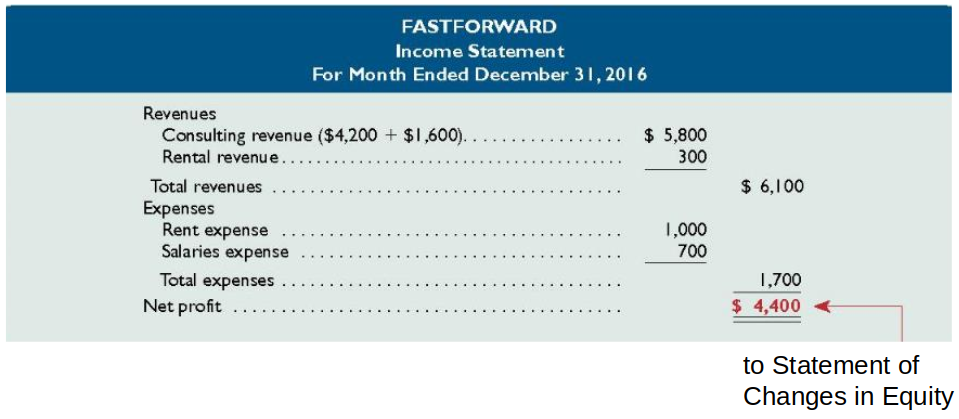
\includegraphics[width=1\columnwidth]{images/c1/income_statement.png}
		\caption{Income Statement}
	\end{figure}
	
	In the income statement, revenues are first reported on the income 
	statement. Expenses are reported after revenues. Net profit (or loss) is 
	reported at the bottom of the statement. 
	
	\subsubsection{Statement of Changes in Equity}
	
	The statement of changes in equity reports information about how equity 
	changes over the reporting period. 
	
	\begin{figure}[ht!]
	\centering
	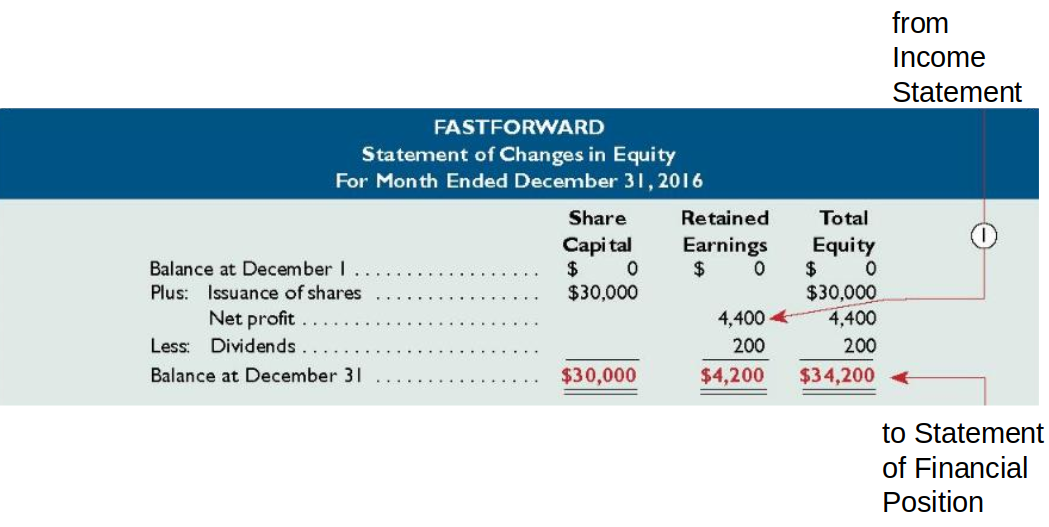
\includegraphics[width=1\columnwidth]{images/c1/financial_sce.png}
	\caption{Statement of Changes in Equity}
	\end{figure}
	
	This statement shows the beginning share 
	capital, events that increase the issuance of shares and net profit), and 
	events that decrease it (dividends and net loss). Cumulative net profit 
	(and loss) not distributed to shareholders are known as retained earnings. 
	
	Ending equity is computed in this statement and it is carried over and 
	reported in the statement of financial position.
	
	\subsubsection{Statement of Financial Position}
	This statement refers to the financial condition at the reporting period. 
	
	\begin{figure}[ht!]
		\centering
		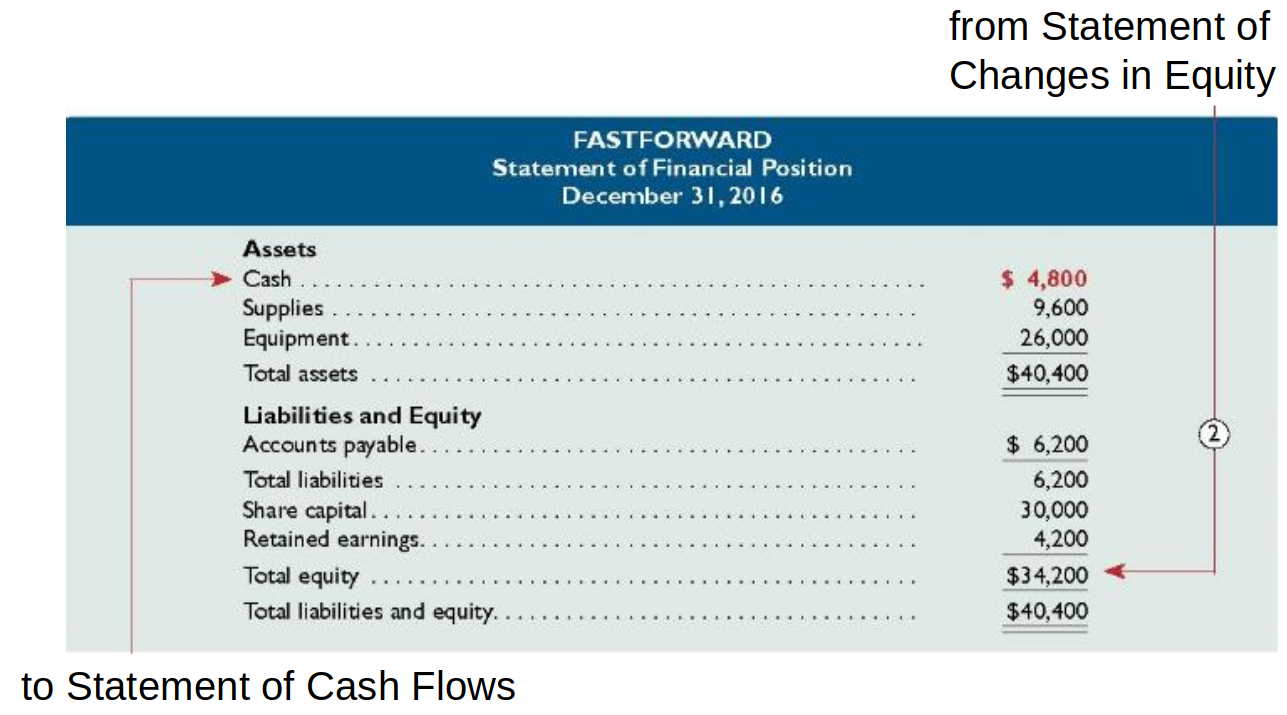
\includegraphics[width=1\columnwidth]{images/c1/statement_of_financial_position.png}
		\caption{Statement of Financial Position}
	\end{figure}
	The top portion lists the assets \ie cash, supplies and other 
	equipment while the next portion shows the liabilities \eg bank loans \etc 
	The equity balance is displayed at the bottom. 
	
	\subsubsection{Statement of Cash Flows}
	
	The statement of cash flows describes a comapny's cash flows for operating, 
	investing and financing activities. 
	\begin{figure}[ht!]
		\centering
		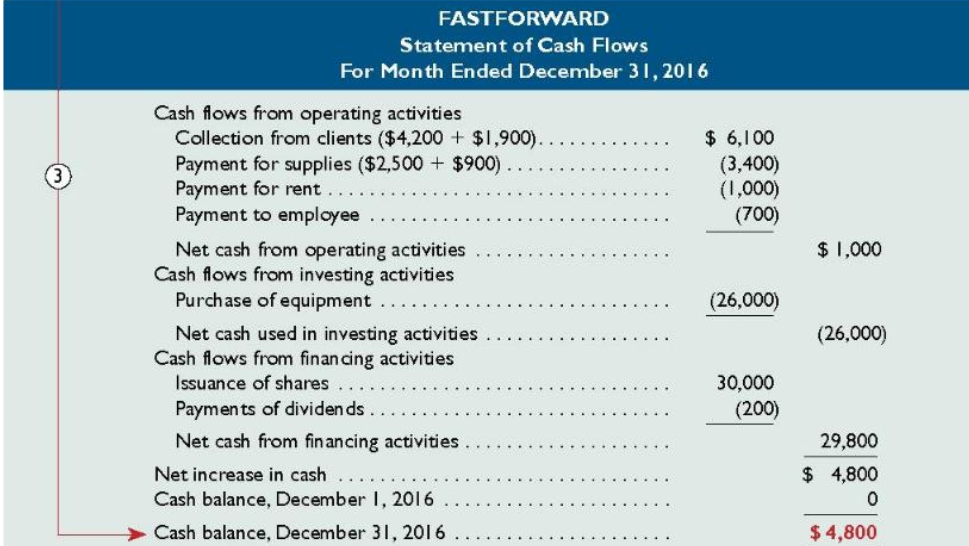
\includegraphics[width=1\columnwidth]{images/c1/statement_of_cash_flows.png}
		\caption{Statement of Cash Flows}
	\end{figure}
	
	Outflows are parentheses to denote subtraction. If cash paid exceeds cash 
	received, we call it 'cash used in operating activities'. The second 
	section reports investing activities, which involve buying and selling 
	assets \eg land and equipment that are held for long-term year (typically 
	more than a year). The third section shows cash flows from financing 
	activities which include long-term borrowing and repaying of cash from 
	lenders and cash from share issuance, and payment of dividends to 
	shareholders. 
	
	
	\subsubsection{Return and Risk Analysis}
	
	Net profit is often linked to \textbf{return}. \textbf{Risk} is the 
	uncertainty about the return we will earn. All business investments involve 
	risk, but some investments involve more risk than others. The lower the 
	risk of an investment, the lower is our expected return. 
	
	The trade-off between return and risk is a normal part of business. Higher 
	risk implies higher, but riskier, expected returns. To help us make better 
	decisions, we use accounting information to assess both return and risk \eg 
	The reason that savings accounts pay such a low return is the low risk of 
	not being repaid with interest. If we buy a share of Adidas or any other 
	company, we might obtain a large return. However, we have no guarantee of 
	any return; there is even the risk of loss.
	
\end{document}